\documentclass[../../main.tex]{subfiles}
\begin{document}

{\bf [解]}
題意より
\begin{align}
 0<t\le\dfrac{1}{2} \label{eq:1}
\end{align}
で考える．与えられた放物線を
\begin{align}
 y=f(t)=\dfrac{1}{2}\left\{t+\dfrac{x(2-x)}{t}\right\} \label{eq:2}
\end{align}
とおく．\cref{eq:1}の端点での値は
\begin{align}
 f\left(\dfrac{1}{2}\right)   = -x^2+2x+\dfrac{1}{4}=-(x-1)^2+\dfrac{5}{4} \label{eq:3}
\end{align}
であり，$t\to +0$での値は$x(x-2)$の符号に応じて変化する．


一階微分は
\begin{align}
f'(t)=\dfrac{1}{2}\left\{1+\dfrac{x(x-2)}{t^2}\right\} \label{eq:4}
\end{align}
であり，この増減表は$x$の値によって以下のように場合分けできる．



\subparagraph{$1^\circ$ $x\le0,\ 2\le x$の時}

この時は\cref{eq:4}より$f'(t)>0$となって，$f(t)$は単調増加である．
またこの時$x(2-x)<0$だから
\begin{align}
 \lim_{t\to +0}f(t) = -\infty 
\end{align}
である．
従って\cref{eq:2}より\cref{eq:1}の範囲では
\begin{align}
 \lim_{t\to0}f(t)<y\le f\left(\dfrac{1}{2}\right) \\
\therefore
  y\le f\left(\dfrac{1}{2}\right) \label{eq:5}
\end{align}
となる．

\subparagraph{$2^\circ$ $0<x<1-\dfrac{\sqrt{3}}{2},\ 1+\dfrac{\sqrt{3}}{2}<x<2$の時}

この時$f(t)$の増減表は以下のようになる．
\begin{table}[htb]
\begin{center}
\begin{tabular}{c|ccccc}
$t$ & $0$ & & $\sqrt{x(2-x)}$ & & $\dfrac{1}{2}$ \\
\hline
$f'$ & & $-$ & $0$ & $+$ & \\
\hline
$f$ & & $\searrow$ & & $\nearrow$ &
\end{tabular}
\end{center}
 \end{table}

またこの範囲では$x(2-x)>0$だから\cref{eq:3}と合わせて
\begin{align}
 \lim_{t\to +0}f(t) =\infty > f\left(\dfrac{1}{2}\right)
\end{align}
であり，また
\begin{align}
 f(\sqrt{x(2-x)})=\sqrt{x(2-x)}
\end{align}
である．従って$y=f(t)$の動く範囲は
\begin{align}
 f(\sqrt{x(2-x)})\le f(t)<\lim_{t\to0}f(t) \\ 
\therefore 
 \sqrt{x(2-x)} \le y \label{eq:6}
\end{align}
である．

\subparagraph{$3^\circ$ $1-\dfrac{\sqrt{3}}{2}\le x\le1+\dfrac{\sqrt{3}}{2}$の時}

この時は\cref{eq:4}から$f'(t)<0$であって，$f(t)$は単調減少である．
またこの時$x(2-x)<0$より
\begin{align}
 \lim_{t\to +0} f(t) = \infty
\end{align}
である．
従って\cref{eq:1}の範囲では
\begin{align}
 f\left(\dfrac{1}{2}\right)\le y <\lim_{t\to +0}f(t)=\infty \\
\therefore
 f\left(\dfrac{1}{2}\right)\le y \label{eq:7}
\end{align}
である．

以上の場合分けをまとめると\cref{eq:5,eq:6,eq:7}より求める領域は以下のようになる．
\begin{align}
 \begin{cases}
   y\le -(x-1)^2+\dfrac{5}{4}  & \left( x\le0,\ 2\le x\right)  \\
   \sqrt{x(2-x)} \le y         & \left( 0<x<1-\dfrac{\sqrt{3}}{2},\ 1+\dfrac{\sqrt{3}}{2}<x<2\right) \\
   -(x-1)^2+\dfrac{5}{4} \le y & \left( 1-\dfrac{\sqrt{3}}{2}\le x\le1+\dfrac{\sqrt{3}}{2}\right) 
 \end{cases}
\end{align}
これを図示すると下図の斜線部となる．境界は$x=0,2$を除く．

\begin{figure}[htb]
\begin{center}
\begin{tikzpicture}[scale=1.0, >=stealth]
  % 座標軸
  \draw[->] (-1.6,0) -- (3.6,0) node[right] {$x$};
  \draw[->] (0,-1.6) -- (0,2.3) node[above] {$y$};
  % 2° (0<x<1-sqrt3/2, 1+sqrt3/2<x<2): 包絡線 y=sqrt(x(2-x)) から上方
  \begin{scope}
    \clip (0,0) rectangle (0.134,2.3);
    \fill[gray!25] plot[domain=0:0.134,samples=20] (\x,{sqrt(\x*(2-\x))}) -- (0.134,2.3) -- (0,2.3) -- cycle;
  \end{scope}
  % 3° (1-sqrt3/2<=x<=1+sqrt3/2): 包絡線 y=-(x-1)^2+5/4 から上方
  \begin{scope}
    \clip (0.134,0) rectangle (1.866,2.3);
    \fill[gray!25] plot[domain=0.134:1.866,samples=40] (\x,{-(\x-1)*(\x-1)+1.25}) -- (1.866,2.3) -- (0.134,2.3) -- cycle;
  \end{scope}
  \begin{scope}
    \clip (1.866,0) rectangle (2,2.3);
    \fill[gray!25] plot[domain=1.866:2,samples=20] (\x,{sqrt(\x*(2-\x))}) -- (2,2.3) -- (1.866,2.3) -- cycle;
  \end{scope}
  % 1° (x<=0, 2<=x): 放物線 y=-(x-1)^2+5/4 から下方
  \begin{scope}
    \clip (-1.6,-1.6) rectangle (0,2.3);
    \fill[gray!25] (-1.6,-1.6) -- (0,-1.6) plot[domain=0:-1.6,samples=20] (\x,{-(\x-1)*(\x-1)+1.25}) -- cycle;
  \end{scope}
  \begin{scope}
    \clip (2,-1.6) rectangle (3.6,2.3);
    \fill[gray!25] (2,-1.6) -- (3.6,-1.6) -- (3.6,{-(3.6-1)*(3.6-1)+1.25}) plot[domain=3.6:2,samples=20] (\x,{-(\x-1)*(\x-1)+1.25}) -- cycle;
  \end{scope}
  \draw[domain=0:2, smooth, thick] plot (\x,{sqrt(\x*(2-\x))});
  \draw[domain=-1.6:3.6, smooth, thick] plot (\x,{-(\x-1)*(\x-1)+1.25});
  \draw[dashed] (0.134,-1.6) -- (0.134,2.3);
  \draw[dashed] (1.866,-1.6) -- (1.866,2.3);
  \node[below] at (0.134,-1.6) {$1-\dfrac{\sqrt{3}}{2}$};
  \node[below] at (1.866,-1.6) {$1+\dfrac{\sqrt{3}}{2}$};
\end{tikzpicture}
\end{center}
\caption{条件を満たす領域の図示（斜線部）}
\end{figure}
（$0<x<2$の部分は上側の曲線・放物線の下側包絡線から上方に無限に広がる領域，$x\le0,2\le x$の部分は放物線$y=-(x-1)^2+\dfrac{5}{4}$の下方に無限に広がる領域．灰色部は図の枠内で切り取って表示している．）

\begin{figure}[htb]
\begin{center}
\begin{tikzpicture}[scale=3, >=stealth, every node/.style={font=\small}]

  % --- 1. 斜線塗りつぶし (領域 E) ---
  
  % [中央領域] 0 < x < 2 における上部領域
  % x in (0, 0.134) : 半円 y = sqrt(x(2-x)) より上
  % x in (0.134, 1.866) : 放物線 y = -(x-1)^2 + 5/4 より上
  % x in (1.866, 2) : 半円 y = sqrt(x(2-x)) より上
  \fill[pattern=north east lines, pattern color=black!50]
    (0, 2.2) -- (0, 0) 
    -- plot[domain=0:0.134, samples=30] (\x, {sqrt(\x*(2-\x))})
    -- plot[domain=0.134:1.866, samples=30] (\x, { -(\x-1)*(\x-1) + 1.25 })
    -- plot[domain=1.866:2, samples=30] (\x, {sqrt(\x*(2-\x))})
    -- (2, 2.2) -- cycle;

  % [左側領域] x <= 0 において放物線より下
  \fill[pattern=north east lines, pattern color=black!50]
    (0, -1.0) -- (0, 0)
    -- plot[domain=0:-0.5, samples=30] (\x, { -(\x-1)*(\x-1) + 1.25 })
    -- cycle;

  % [右側領域] x >= 2 において放物線より下
  \fill[pattern=north east lines, pattern color=black!50]
    (2, -1) -- (2, 0)
    -- plot[domain=2:2.5, samples=30] (\x, { -(\x-1)*(\x-1) + 1.25 })
    -- cycle;

  % --- 2. 補助線（点線） ---
  % x = 1 - \sqrt{3}/2 および x = 1 + \sqrt{3}/2 の垂線
  \draw[dashed, gray!70] (0.134, 0) -- (0.134, 0.5) -- (0, 0.5);
  \draw[dashed, gray!70] (1.866, 0) -- (1.866, 0.5);
  
  % 放物線・半円の頂点からの補助線
  \draw[dashed, gray!70] (1, 0) -- (1, 1.25) -- (0, 1.25);

  % --- 3. 座標軸 ---
  \draw[->, thick] (-1, 0) -- (3, 0) node[right] {$x$};
  \draw[->, thick] (0, -1.4) -- (0, 2.5) node[above] {$y$};
  \node[below left] at (0,0) {$O$};

  % --- 4. 曲線・放物線の描画 ---
  % 半円 y = sqrt(x(2-x))
  \draw[domain=0:2, smooth, thick, blue!80!black, samples=60] 
    plot (\x, {sqrt(\x*(2-\x))}) node[blue!80!black, font=\small] {$y=\sqrt{x(2-x)}$};
  
  % 放物線 y = -(x-1)^2 + 5/4
  \draw[domain=-0.5:2.5, smooth, thick, red!80!black, samples=60] 
    plot (\x, { -(\x-1)*(\x-1) + 1.25 }) node[red!80!black, font=\small] {$y=-(x-1)^2+\dfrac{5}{4}$};

  % --- 5. 軸上の目盛りテキスト ---
  \node[below] at (0.134, 0) {\scriptsize $1-\dfrac{\sqrt{3}}{2}$};
  \node[below] at (1.866, 0) {\scriptsize $1+\dfrac{\sqrt{3}}{2}$};
  \node[below] at (1, 0) {$1$};
  \node[below right] at (2, 0) {$2$};

  \node[left] at (0, 0.5) {$\dfrac{1}{2}$};
  \node[left] at (0, 1.25) {$\dfrac{5}{4}$};

  % --- 6. 特徴的な点とプロット（境界除外点の白抜き丸） ---
  % 放物線の頂点 (1, 5/4)
  \fill[red!80!black] (1, 1.25) circle (1.2pt);

  % 交点 (1 \pm \sqrt{3}/2, 1/2)
  \fill (0.134, 0.5) circle (1.2pt);
  \fill (1.866, 0.5) circle (1.2pt);

  % 除外点 x = 0, 2 (白抜き丸)
  \fill (0,0) circle (1.2pt);
  \fill (2,0) circle (1.2pt);

  % 領域のラベル
  \node[fill=white, inner sep=1pt, font=\bfseries] at (1, 1.7) {領域 $E$};

\end{tikzpicture}
\end{center}
\caption{条件を満たす領域の図示（斜線部，境界は $x=0,2$ を除く）}
\end{figure}


\newpage

\end{document}
